\section{Technologies Used}
\label{sec:technologies_used}

This section will outline the technologies used to implement the BT specification detailed in Section \ref{sec:specification}.

\subsection{Behavior Trees Technologies}

\subsubsection{BehaviorTree.CPP}

Implementing a BT engine can be a complex task, therefore, when developing new BTs, the use of existing libraries is highly recommended. The use of libraries ensures greater ease in the development and debugging process, better quality of the developed code and greater support for features, in addition to having a community of developers who can help with software problems.

Regarding the use of libraries for developing BTs in robotics applications, there are two libraries that stand out \cite{BTsAndFSMApplications}, which are the \textit{BehaviorTree.CPP} \cite{BehaviorTree.CPP} and the \textit{PyTrees} \cite{PyTrees}. Both of these libraries have a huge community, many features and great documentation pages.

As mentioned in Section \ref{sec:organization_model}, the ThunderVolt project already employed BTs, but for the implementation of the behaviors of the individual roles that the robots can play. In an older version of the project \cite{fira_thundervolt}, the team used the \textit{PyTrees} library to define the behavior of the roles, however, due to the computational intensity required by the project, the team had performance problems when using this library, which impaired its real-time reactivity. Therefore, as suggested by the \textit{PyTrees} documentation itself \cite{PyTreesDesign}, instead of using Python to model the trees, the team chose to migrate to the C++ language, in order to increase the system performance, hence the \textit{BehaviorTree.CPP} was used in that context.

The \textit{BehaviorTree.CPP} library presents a C++ framework to create BTs, providing tools that help develop many different and complex trees, extending the basic functionalities that BTs support. The library is an open-source project, which was initially maintained by the author of \cite{BTsInRobotics} and now is mainly maintained by Davide Faconti\footnote{https://github.com/facontidavide}.

The \textit{BehaviorTree.CPP} library offers many features such as built-in nodes that simplify the process of implementing BTs, easy access to a well structured blackboard, asynchronous nodes, and many others. In addition, to enhance the development and debugging process of implementing BTs, the library provides a logging and profiling infrastructure to, for example, visualize and record the state transitions of the tree. Furthermore, one of its main advantages is the ability to describe trees using an interpreted language based on XML and create the trees dynamically during run-time, making the development process of the tree much faster, as changes in the tree can be easily implemented and tested.

Thus, this library presented itself as a great candidate to be used in the development of the new strategy for many reasons. One of the first reasons is the prior experience with the library, which significantly facilitated its usage for implementing the new strategy and provided an opportunity to evaluate the library's compatibility with the project's requirements. Besides that, the library presents many functionalities that are useful for the specified tree, in addition to being an open-source project, having a large community of developers using and supporting it and being extensively used in very diverse and important robotics applications, such as the Navigation 2 \cite{nav2} ROS package.

Finally, it is important to mention that the tree was implemented with version 3.8 of the library, which was the latest version at the time of its development. There are already newer versions of the library, but changing to these newer versions would not impact the structure of the presented tree.

\subsubsection{Groot}
\label{subsubsec:groot}

When it comes to building and debugging BTs, having a visual tool that allows visualizing the tree structure and facilitates tracking the execution flow of the tree proves to be immensely beneficial. Hence, another tool compliant with the \textit{BehaviorTree.CPP} library was developed by Davide Faconti, called \textit{Groot} \cite{Groot}.

\textit{Groot} is an integrated development environment for BTs that were developed with \textit{BehaviorTree.CPP}, offering the possibility to visually edit and export trees, record the execution flow of a tree in a log file and replay it afterward, and monitor each tick of the tree in real-time.

This tool is one of the other advantages of using the \textit{BehaviorTree.CPP} library and was used during the whole process of development and debugging of the new strategy.

It is important to note that there are two versions of \textit{Groot} currently available. The first version is an open-source project, compatible with version 3.8 of the \textit{BehaviorTree.CPP} library and unfortunately it is being deprecated at the moment. The second version of \textit{Groot} has more advanced functionalities and it supports version 3.8 and versions equal to or higher than 4.2 of the library, however, it is no longer an open-source project and most of its features require a paid license.

\begin{figure}[h]
    \centering
    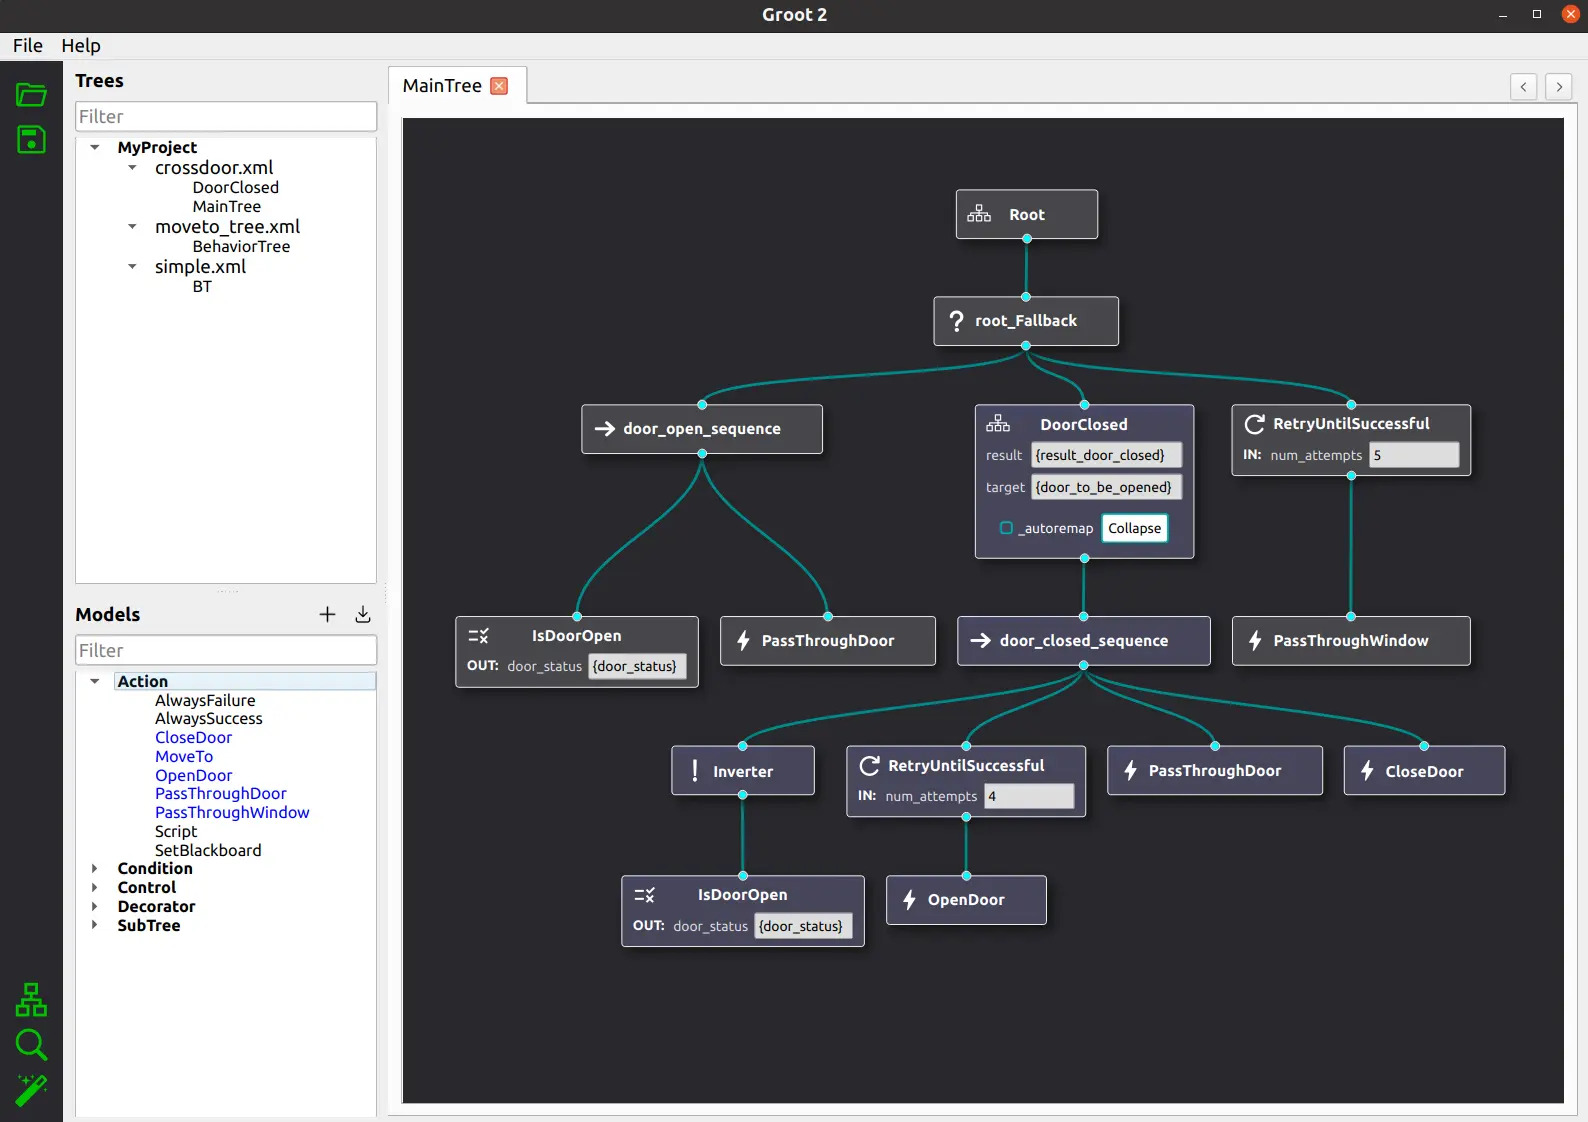
\includegraphics[width=0.75\linewidth]{chapters/development/images/Groot.jpg}
    \caption{Groot 2 interface. Taken from \cite{Groot}}
    \label{fig:groot}
\end{figure}

\subsection{Auxiliary Technologies}

In addition to the technologies used to build and debug the trees, other technologies are utilized in the context of the tree's operation, which will be elucidated as follows. These technologies were not chosen during the development of the new strategy, they were already employed by the ThunderVolt project and are part of its architecture as a whole.

Within this Subsection, these other technologies will be presented and their integration within the tree will be elucidated. This detailed explanation aims to facilitate a comprehensive understanding of how the tree is integrated with the rest of the system.

\subsubsection{Protobuf and UDP}

In the VSSS category, there are two tools that are important when testing and playing games, which are the FIRASim simulator, and the VSSReferee, the automatic referee system. Both of these systems are crucial for the operation of the tree, as the simulator sends the states of the robots, which are used to decide when the roles of the robots should change, and the referee sends the events that define when the \texttt{Roles Swapper Initializer} tree (defined in Subsection \ref{subsec:roles_swapper_initializer_spec}) should be executed and how the initialization should be performed.

In order to be able to communicate with those two systems, a protocol was defined by the category \cite{VSSProto} using Google's Protocol Buffers (\textit{Protobuf}) \cite{Protobuf}. \textit{Protobuf} is a language-neutral and cross-platform framework to serialize data, so it can be stored or sent over a network. In the use case of the category, the serialized data is exchanged between the simulator, the referee and the teams playing the game using the User Datagram Protocol (UDP) \cite{rfc768}. UDP is one of the core communication protocols of the internet, being a transaction oriented protocol, meaning that it does not require the network nodes to establish a connection to be able to communicate with each other. For the UDP-based communication, the team leveraged the capabilities of the \textit{Boost.Asio} library \cite{BoostAsio}, which is a cross-platform C++ library for network communication.

\subsubsection{ROS}

The Robot Operating System (\textit{ROS}) \cite{ROS} is a framework for developing robotics applications, it offers a diverse set of libraries and tools that help to build robotics projects. \textit{ROS} has a very large and global community, which helps to maintain all the libraries and to develop new algorithms, drivers and tools for the framework.

In the ThunderVolt project, \textit{ROS} is used to compose the structure of the whole software application, defining how the project will be executed, specifying the communication interface between all the different parts of the project that are performed in parallel, in addition to helping the system to be easily configured and calibrated. In a less abstract way, for example, it is through ROS that the coordination strategy that is running in a separate process publishes the roles of the robots to the other processes that represent the robots, so they can execute the correct behavior.
